\documentclass[14pt]{beamer} 
\usetheme{default}

\usepackage{import}
\usepackage{graphicx}
\usepackage{amsmath}
\usepackage{amssymb}
\usepackage{amsthm}

\usepackage{tikz}
\usetikzlibrary{arrows}
\usetikzlibrary{shapes, arrows.meta}

\usepackage{pgfplots}
\usepackage[T1]{fontenc}
\usepackage{lmodern}
\usepackage[utf8]{inputenc}

\usepackage{caption}
\usepackage{subcaption}
\usepackage{../tex/mathpartir}

%\setbeamercovered{transparent}
\definecolor{bgcol}{rgb}{0.8, 0.8, 0.8}
\setbeamercolor{bgcolor}{fg=black,bg=bgcol}

\newcommand{\Type}{\mathsf{Type}}
\newcommand{\Space}{\mathsf{Space}}
\newcommand{\Open}{\mathsf{Open}}
\newcommand{\PLower}{\mathcal{P}_\lozenge^+}
\newcommand{\PUpper}{\mathcal{P}_\square^+}
\newcommand{\Prob}{\mathcal{R}}
\newcommand{\State}{\mathsf{State}}

\newcommand{\cov}{\vartriangleleft}
\newcommand{\nat}{\mathbb{N}}
\newcommand{\suchthat}{\ |\ }
\newcommand{\List}[1]{\mathsf{list}\ {#1}}
\newcommand{\rat}{\mathbb{Q}}
\newcommand{\R}{\mathbb{R}}
\newcommand{\bool}{\mathbb{B}}
\newcommand{\Prop}{\mathbb{P}}
\newcommand{\Dist}[1]{\mathcal{P}({#1})}
\newcommand{\fun}[2]{\lambda\ {#1}\Rightarrow{#2}}
\newcommand{\ret}[1]{\mathsf{ret}_{#1}}

\newcommand*\circled[1]{\tikz[baseline=(char.base)]{
            \node[shape=circle,draw,inner sep=2pt,thick] (char) {#1};}}
            
\newcommand{\dirsup}{\mathop{\setlength{\unitlength}{.7em}\raisebox{-.2em}%
    {\begin{picture}(1,1.5)\put(.5,0){\line(-1,3){.48}}
    \put(.5,0){\vector(1,3){.5}}\end{picture}}}} 
            
\newcommand*{\tikzbullet}[2]{%
  \setbox0=\hbox{\strut}%
  \begin{tikzpicture}
    \useasboundingbox (-.25em,0) rectangle (.25em,\ht0);
    \filldraw[draw=#1,fill=#2] (0,0.3\ht0) circle[radius=.25em];
  \end{tikzpicture}%
}

\newcommand{\SafeToGo}{\tikzbullet{green}{green}}
\newcommand{\SafeToStop}{\tikzbullet{red}{red}}

\title{Programming with continuous spaces}
\author{\textbf{Ben Sherman}, Luke Sciarappa, Michael Carbin, Adam Chlipala
\\ \small MIT}
\date{October 7, 2016}

\setbeamertemplate{footline}{}
\setbeamertemplate{navigation symbols}{}
%\setbeamertemplate{headline}
%{\vspace{0.03em}
%\begin{beamercolorbox}[wd=\paperwidth,ht=4ex,dp=1ex,center]{bgcolor}
% \small \insertshorttitle
%  \end{beamercolorbox}
%}
\begin{document}

\maketitle

\begin{frame}
\begin{center}
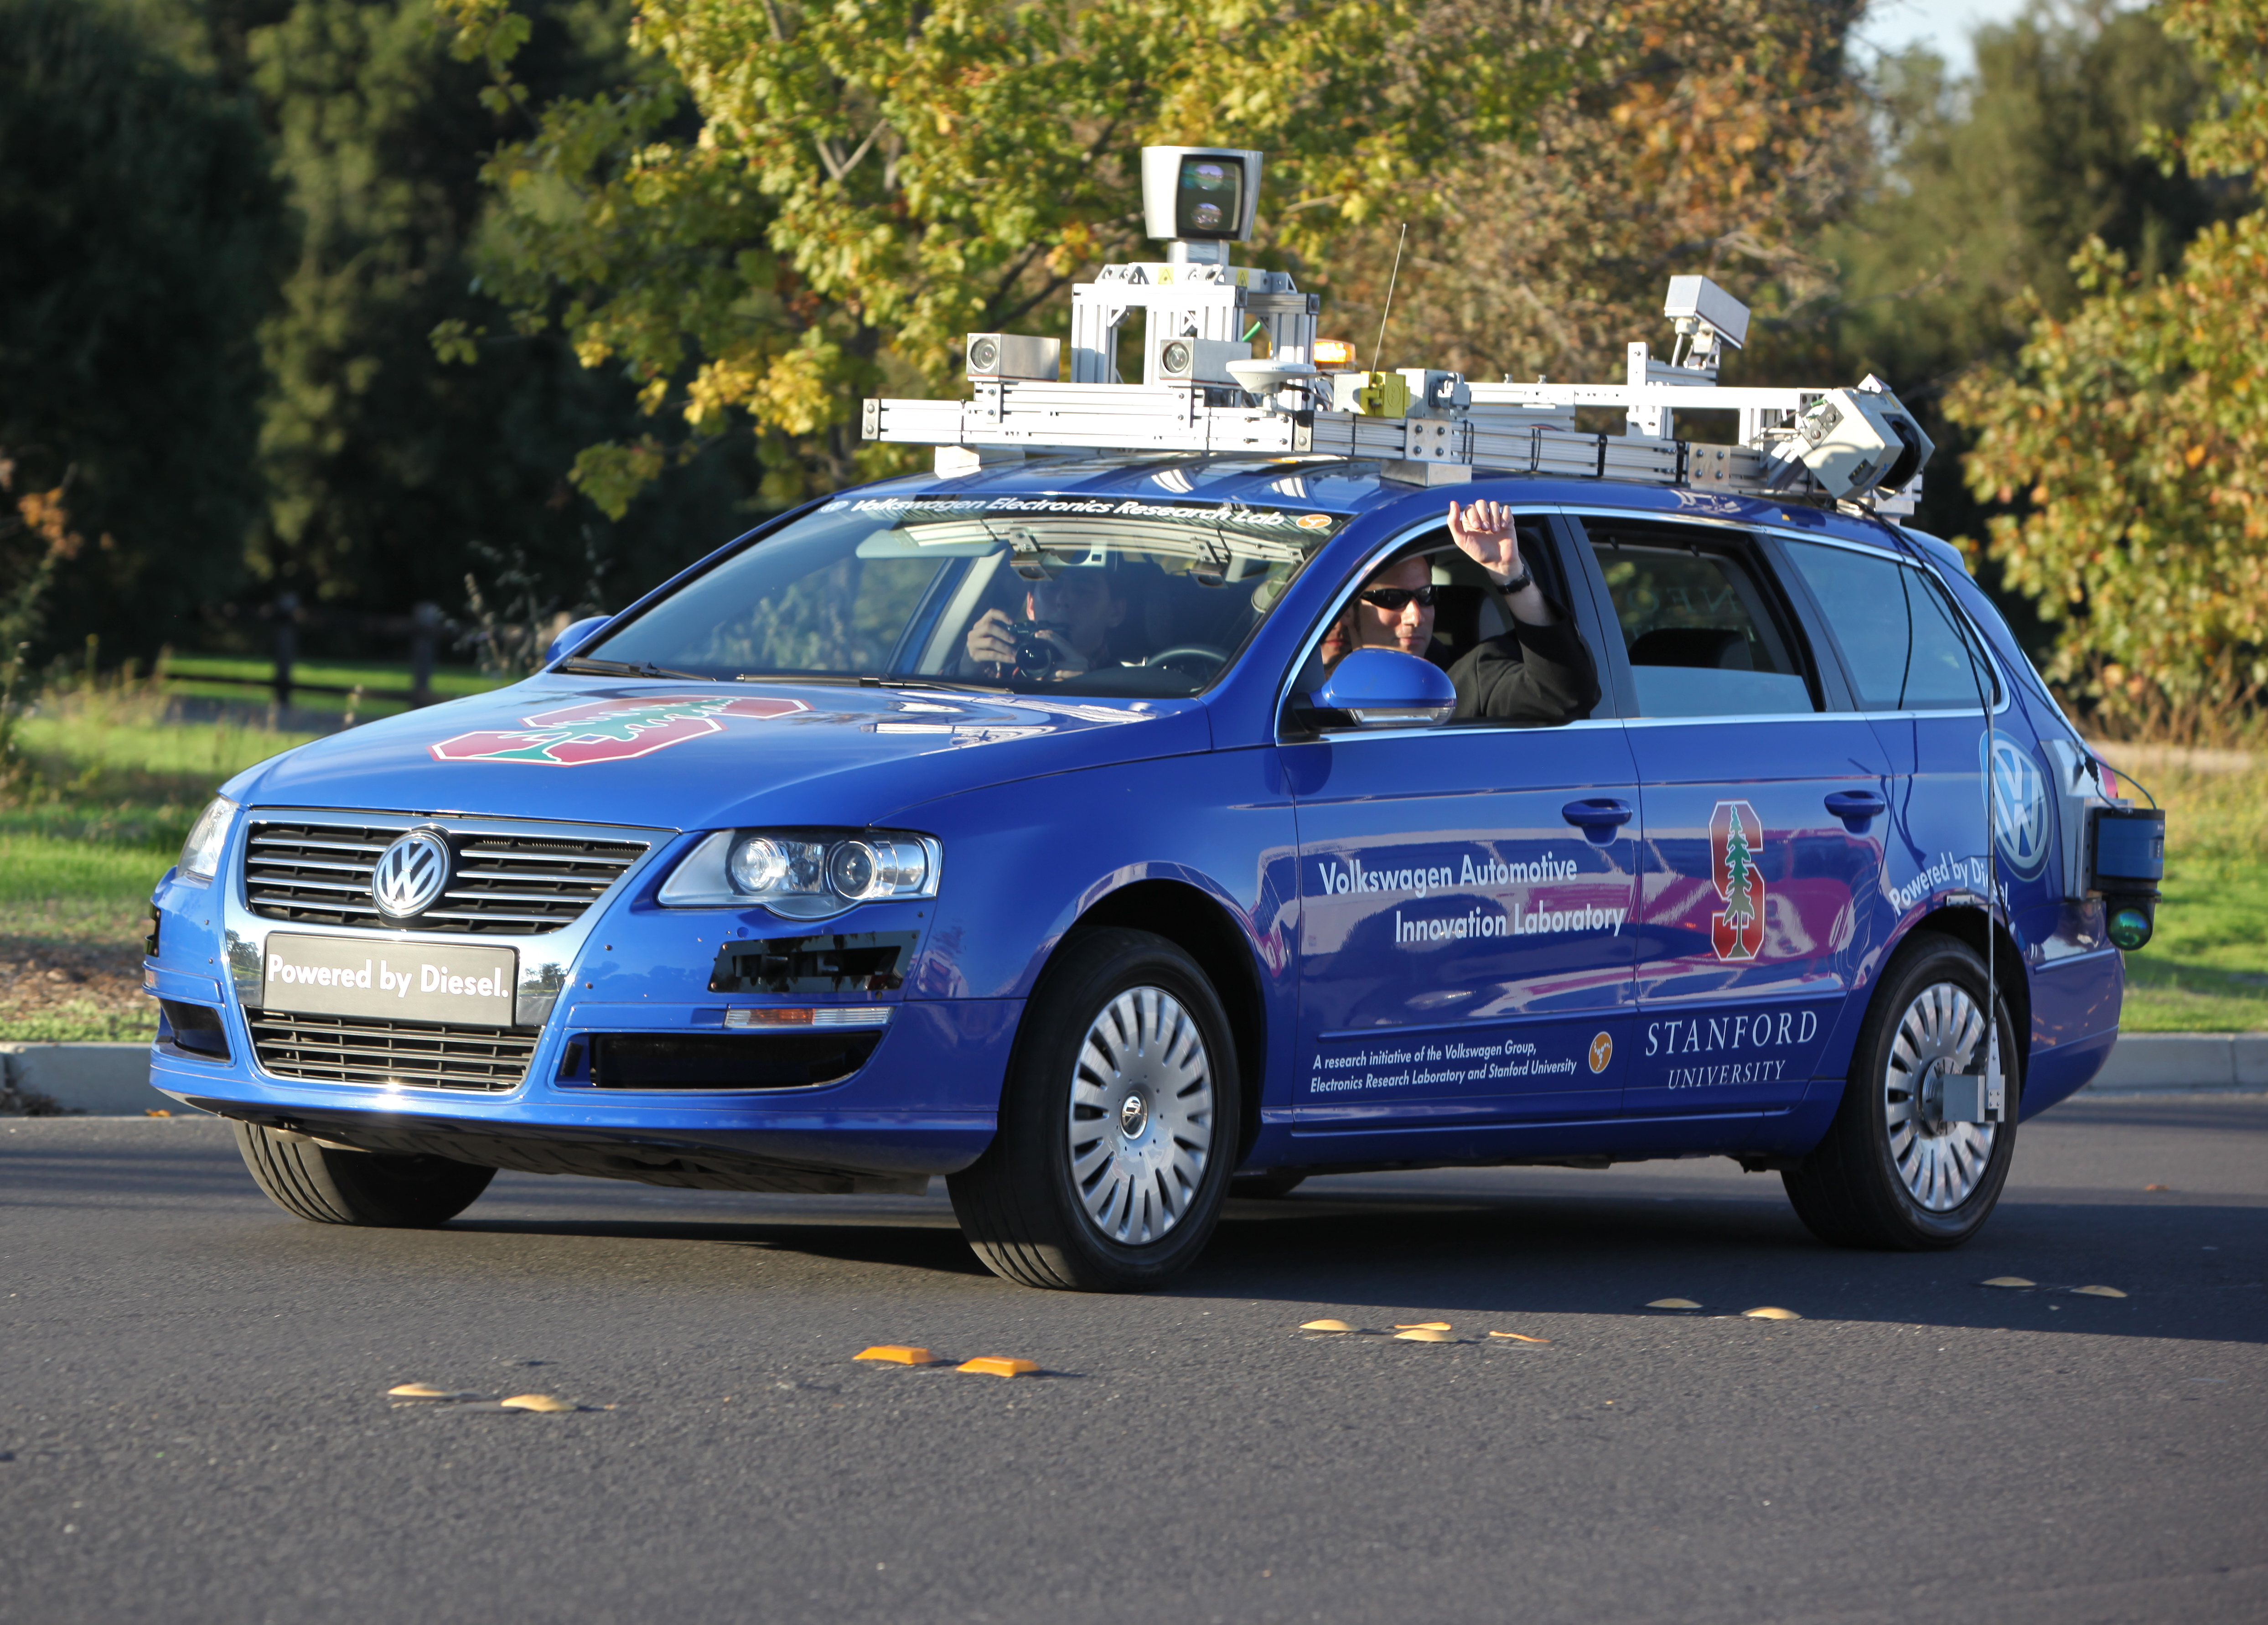
\includegraphics[width=0.6\textwidth]{images/autonomous-car.jpg}
\\
\includegraphics[width=0.6\textwidth]{images/drone.jpg}
\end{center}
\end{frame}

\begin{frame}
A programming language for continuous spaces which
\begin{enumerate}
\item facilitates formal guarantees
% program with mathematical objects themselves. no approximation error or rounding error. Expected algebraic identities hold
\item ensures programs are robust to perturbations
% every program is continuous
\item facilitates reasoning about uncertainty: non-determinism and probability
% non-determinism and randomness are computational. Also monadic. Every space automatically has probabilistic powerspace (not easy to give probabilistic semantics for other programming languages)
\end{enumerate}
\end{frame}

\begin{frame}

\begin{center}
\Large 
\begin{align*}
\text{types} &\triangleq \text{spaces}
\\
\text{open expressions} &\triangleq \text{continuous maps}
\\
\text{closed expressions} &\triangleq \text{points}
\end{align*}
\end{center}
\end{frame}

\begin{frame}{1. Facilitates formal guarantees}
\[
\forall x, y : \R, x + (y - x) = x
\]
\end{frame}

\begin{frame}{2. Is robust to perturbations}
\emph{Continuity and robustness of programs} by Swarat Chaudhuri, Sumit Gulwani, and Robert Lublinerman

Any function $A \to B$ is \emph{automatically} continuous
\end{frame}

\begin{frame}{What is continuity?}
Indiscernible property of inputs $\Rightarrow$ indiscernable property of outputs

Observable property of output $\Rightarrow$ observable property of input
\end{frame}

%\begin{frame}{3. Facilitates reasoning about uncertainty}
%\end{frame}


\begin{frame}{Running points}
\begin{center}
\resizebox{0.7\textwidth}{!}{\import{../Figures/Cover/output/}{step1.pdf_tex}}
\end{center}
\end{frame}

\begin{frame}{Running points}
\begin{center}
\resizebox{0.7\textwidth}{!}{\import{../Figures/Cover/output/}{step2.pdf_tex}}
\end{center}
\end{frame}

\begin{frame}{Running points}
\begin{center}
\resizebox{0.7\textwidth}{!}{\import{../Figures/Cover/output/}{step3.pdf_tex}}
\end{center}
\end{frame}



\begin{frame}
\small
\begin{figure}
\begin{center}
\frame{\begin{subfigure}[t]{\textwidth}
\begin{center}
 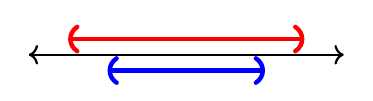
\begin{tikzpicture}
 \node[draw=white] (spacing) at (0, 0.22) {}; %for spacing purposes only
 \draw [<->, thick] (-2, 0) -- (2, 0);
 \draw [(-), ultra thick, blue] (-1, -0.2) -- (1, -0.2);
 \draw [(-), ultra thick, red] (-1.5, 0.2) -- (1.5, 0.2);
 \end{tikzpicture}
 \end{center}
\begin{mathpar}
\inferrule* [right=widen]
  {p' \le p < q \le q' }
  {p < \cdot < q \vdash p' < \cdot < q'}
\end{mathpar}
\end{subfigure}}

\vspace{1em}

\frame{\begin{subfigure}[t]{\textwidth}
\begin{center}
 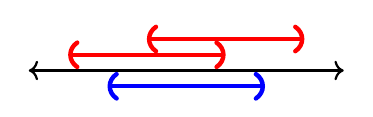
\begin{tikzpicture}
\node[draw=white] (spacing) at (0, 0.42) {}; %for spacing purposes only
 \draw [<->, thick] (-2, 0) -- (2, 0);
 \draw [(-), ultra thick, blue] (-1, -0.2) -- (1, -0.2);
 \draw [(-), ultra thick, red] (-1.5, 0.2) -- (0.5, 0.2);
  \draw [(-), ultra thick, red] (-0.5, 0.4) -- (1.5, 0.4);
 \end{tikzpicture}
 \end{center}
\begin{mathpar}
\inferrule* [right=split]
  {r < p < u < s < q < v}
  {p < \cdot < q \vdash r < \cdot < s \ \vee\  u < \cdot < v }
\end{mathpar}
\end{subfigure}}

\vspace{1em}

\frame{\begin{subfigure}[t]{\textwidth}
\begin{center}
 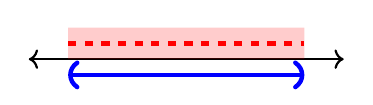
\begin{tikzpicture}
 \draw [<->, thick] (-2, 0) -- (2, 0);
 \draw [(-), ultra thick, blue] (-1.5, -0.2) -- (1.5, -0.2);
 \draw [ultra thick, dashed, red] (-1.5, 0.2) -- (1.5, 0.2);
  \fill[fill=red, opacity=0.2]  (-1.5, 0)--(-1.5,0.4)--(1.5,0.4)--(1.5,0)--(-1.5,0);
 \end{tikzpicture}
 \end{center}
\begin{mathpar}
\inferrule* [right=inside]
  { }
  {p < \cdot < q \vdash \bigvee \{ x < \cdot < y \suchthat p < x < y < q \}}
\end{mathpar}
\end{subfigure}}

\end{center}
\end{figure}
\end{frame}

\begin{frame}{Running points (formally)}
\begin{align*}
&A : \Space \\
& I : \Type \\
&i : I \vdash P_i : \Open(A) \\
&x : \mathsf{Pt}(A)
\end{align*}

\bigskip

\begin{mathpar}
\inferrule* [right=]
  {\quad \top \vdash_A \bigvee_{i : I} P_i}
  {\exists i : I, x \models P_i}
\end{mathpar}
\end{frame}

\begin{frame}{Example computation rules}
\begin{mathpar}
\inferrule* [right=]
  {\varepsilon : \rat^+}
  {\top \vdash_\R \bigvee_{q : \rat} q - \varepsilon < \cdot < q + \varepsilon}
\end{mathpar}

\begin{mathpar}
\inferrule* [right=]
  {\top \vdash_A \bigvee_{i : I} P_i
  \\ \top \vdash_B \bigvee_{j : J} Q_j}
  {\top \vdash_{A \times B} \bigvee_{(i, j) : I \times J} P_i \times Q_j}
\end{mathpar}

\end{frame}

\begin{frame}{Example computation rules (simplified)}
\[
\Downarrow : \Space \to \Type \to \Type
\]

\begin{mathpar}
\inferrule* [right=]
  {\varepsilon : \rat^+}
  {\R \Downarrow \rat}
\end{mathpar}

\begin{mathpar}
\inferrule* [right=]
  {A \Downarrow I
  \\ B \Downarrow J}
  {A \times B \Downarrow I \times J}
\end{mathpar}

\end{frame}

\begin{frame}{Buridan's principle}
\begin{center}
\Huge $\R \to \bool$
\\
\includegraphics[width=\textwidth]{images/buridan.jpg}
\end{center}
\end{frame}

\begin{frame}{Buridan's principle}
\begin{center}
\Huge $\R \to \PLower(\bool)$
\\
\includegraphics[width=\textwidth]{images/buridan.jpg}
\end{center}
\end{frame}

\begin{frame}{Simulating non-determinism}
\begin{mathpar}
\inferrule* [right=]
  {\top \vdash_A \bigvee_{i : I} P_i}
  {\top \vdash_{\PLower(A)} \bigvee_{i : I} \lozenge P_i}
\end{mathpar}
\end{frame}

\begin{frame}{Buridan's autonomous car}
\begin{center}
 \begin{tikzpicture}
 \draw [<->, ultra thick] (-5, 0) -- (5, 0);
 \draw [(->, ultra thick, green] (-2, 0.2) -- (5, 0.2);
 \draw [<-), ultra thick, red] (-5, 0.4) -- (2, 0.4);
 \node[inner sep=0pt, anchor=south] (car) at (-2.5, 0.6)
    {\includegraphics[width=.25\textwidth]{images/car.png}};
 \node[inner sep=0pt, anchor=south] (light) at (3.5,0.6)
    {\includegraphics[width=.1\textwidth]{images/traffic-light.png}};
 \end{tikzpicture}
 \end{center}
\end{frame}

\begin{frame}{No input uncertainty}
\begin{align*}
\mathsf{decide} &: \{ \State \suchthat \SafeToGo \vee \SafeToStop \} \to \PLower(\bool)
\\ \mathsf{decide}(s) &= \mathsf{cases}(s)
\begin{cases}
\SafeToGo
  \quad &\Longrightarrow \quad
  \ret{\PLower}(\mathsf{true})
\\
\SafeToStop
  \quad &\Longrightarrow \quad
  \ret{\PLower}(\mathsf{false})
\end{cases}
\end{align*}
\end{frame}

\begin{frame}{Non-determistic input uncertainty}
\begin{align*}
\mathsf{decide} &: \{ \PUpper(\State) \suchthat \square \SafeToGo \vee \square \SafeToStop \} \to \PLower(\bool)
\\ \mathsf{decide}(s) &= \mathsf{cases}(s)
\begin{cases}
\square \SafeToGo
  \quad &\Longrightarrow \quad
  \ret{\PLower}(\mathsf{true})
\\
\square \SafeToStop
  \quad &\Longrightarrow \quad
  \ret{\PLower}(\mathsf{false})
\end{cases}
\end{align*}
\end{frame}

\begin{frame}{Probabilistic uncertainty}
\begin{align*}
\mathsf{decide} &: \{ \Prob(\State) \suchthat \Pr[\SafeToGo] > 99\% \vee \Pr[\SafeToStop] > 99\% \} 
\\ &\to \PLower(\bool)
\\ \mathsf{decide}(s) &= \mathsf{cases}(s)
\begin{cases}
\Pr[\SafeToGo] > 99\%
   &\Longrightarrow
  \ret{\PLower}(\mathsf{true})
\\
\Pr[\SafeToStop] > 99\%
   &\Longrightarrow
  \ret{\PLower}(\mathsf{false})
\end{cases}
\end{align*}
\end{frame}

\begin{frame}{3. Facilitates reasoning about uncertainty}
\begin{itemize}
\item \emph{Every} space has a probabilistic powerspace
\item Non-determinism and randomness have computational meaning
\end{itemize}
\end{frame}

\begin{frame}
\begin{center}
\Huge Questions?

\vspace{3em}

\small Ben Sherman
\\ sherman@csail.mit.edu
\end{center}
\end{frame}

\begin{frame}{Overlapping pattern match semantics}
\begin{mathpar}
\inferrule* [right=]
  {A, B : \Space \\
I : \Type \\
i : I \vdash P_i : \Open(A) \\
i : I \vdash f_i : \{ A \suchthat P_i \} \to B \\
Q : \Open(B) \\
x : \mathsf{Pt}(A) \\
\top \vdash_A \bigvee_{i : I} P_i \\
\forall i, j : I, \exists f_{i,j} : \{ A \suchthat P_i \wedge P_j \} \to B, f_{i,j} = \max(f_i, f_j)
}
  {f(x) \triangleq  \dirsup \{ f_i(x) \suchthat x \models P_i \}}
\end{mathpar}

%should I write this as a directed sup instead? It will likely be unclear no matter what

\[
f(x) = \mathsf{cases}(x) \begin{cases}P_i \Longrightarrow f_i(x) \end{cases}
\]

\end{frame}


\begin{frame}

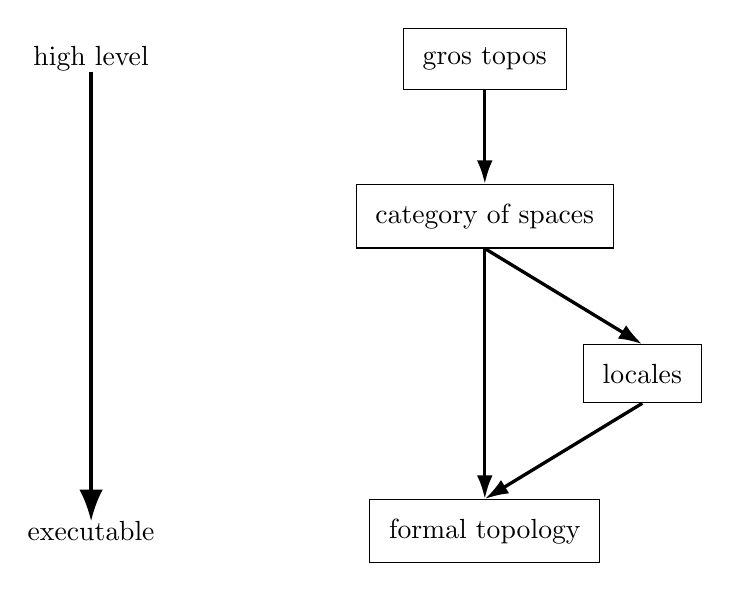
\begin{tikzpicture}
\node[inner sep=0pt] (highlevel) at (0,0)
  {high level};
\node[inner sep=0pt] (executable) at (0, -6)
  {executable};
\draw[-{Latex[length=4mm, width=3mm]},very thick] (highlevel.south) -- (executable.north);

\node[draw=black, rectangle, inner sep=7pt] (topos) at (5,0)
  {gros topos};
\node[draw=black, rectangle, inner sep=7pt] (cat) at (5,-2)
  {category of spaces};
\node[draw=black, rectangle, inner sep=7pt] (loc) at (7,-4)
  {locales};
\node[draw=black, rectangle, inner sep=7pt] (ft) at (5,-6)
  {formal topology};
  
\draw[-{Latex[length=3mm, width=2mm]},very thick] (topos.south) -- (cat.north);
\draw[-{Latex[length=3mm, width=2mm]},very thick] (cat.south) -- (loc.north);
\draw[-{Latex[length=3mm, width=2mm]},very thick] (cat.south) -- (ft.north);
\draw[-{Latex[length=3mm, width=2mm]},very thick] (loc.south) -- (ft.north);

\end{tikzpicture}


\end{frame}


\end{document}

